\chapter{The structure and kinematics of the Milky Way}
In this chapter we describe how SALSA can be used to measure the structure
and kinematics of the Milky Way. First we explain how to measure the rotation curve,
i.e. the rotational speed of the gas at different distances from the galactic center. 
Then we build on these results to make a map of the spiral arms.

\section{The rotation curve of the Milky Way}
A rotation curve is function which describes the rotational speed of the galaxy
at different distances from the center, usually denoted $V(R)$. 
To construct a rotation curve we first need to understand how the velocity we
measure (through Doppler shift) is related to the movement of gas clouds in the
Milky Way. Let us imagine that we point our radio telescope towards a gas cloud
in the Galaxy, i.e. we observe along the green line in Fig. \ref{fig:galgeom}.
\begin{figure}[ht]
\begin{center}
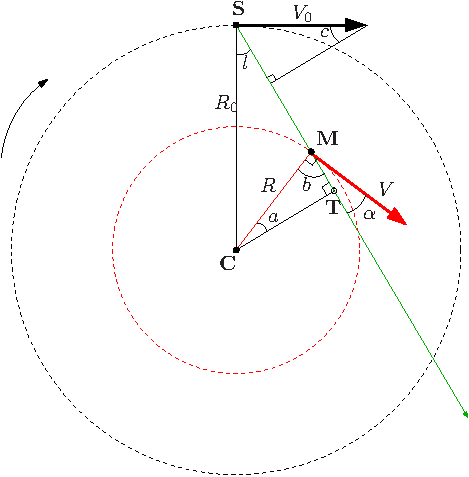
\includegraphics[width=8cm]{../figures/galgeom.pdf}
\end{center}
\caption{Geometry of the Galaxy. {\bf C} is the location of the Galactic center, 
{\bf S} that of the Sun, {\bf M} that of a gas cloud that we want to observe. 
The SM line is the line-of-sight. The arrow on an arc indicates the direction 
of rotation of the Galaxy. The arrows on line segments indicate the
velocity of the Sun ($V_0$) and the gas cloud ($V$).}
\label{fig:galgeom}
\end{figure}  
For future reference we list some variables used in this figure:
\begin{displaymath}
	\boxed{
\begin{array}{ll}
	V_0 	&\hbox{Sun's velocity around the Galactic center, i.e. 220 km/s}					\\
    R_0	&\hbox{Distance of the Sun to the Galactic center, i.e. 8.5 kpc}) 					\\
l	&\hbox{Galactic longitude of observation}				\\
V	&\hbox{Velocity of a cloud of gas}			\\
R	&\hbox{Cloud's distance to the Galactic center}		\\
\end{array}
}
\end{displaymath}

There may be many clouds in this direction, but for the purpose of this
derivation we only care about a single cloud located at position $M$ in Fig.
\ref{fig:galgeom}. Since both the Sun and the cloud are moving, we do not measure
the cloud velocity directly. Instead, we measure the relative velocity, $V_r$,
between the us and the cloud, projected on the line-of-sight.  Using the angles
in Fig. \ref{fig:galgeom} we can write this down as 
\begin{equation}
V_r = V \cos\alpha - V_0 \sin c .
\label{eqn:vrel1}
\end{equation}
For this expression to be useful we need to relate the angles to the galactic
coordinates we discussed in Sect. \ref{sect:galcoords}.  We know that
the sum of angles in the upper right triangle must be 180$^\circ$, which means that 
we can relate the angle $c$ to galactic longitude $l$ as
\begin{equation}
(90-l)+90+c=180 \quad \Rightarrow \quad c=l.
\label{eqn:c}
\end{equation}
We now want to relate $\alpha$ to the longitude $l$. Looking at the
triangles {\bf CST} and {\bf CMT} we find that the distance between the
Galactic Center ({\bf C}) and the tangential point ({\bf T}) can be expressed
in two different ways: 
\begin{equation}
	{\rm\bf CT} = R_0\sin l = R \cos\alpha \quad \Rightarrow \quad \cos \alpha = \frac{R_0\sin l}{R}
\label{eqn:cosalpha}
\end{equation}
Using eqns. \ref{eqn:c} and \ref{eqn:cosalpha} we can now re-write eqn. \ref{eqn:vrel1} as
\begin{equation}
\boxed{V_r = V \frac{R_0}{R}\sin l - V_0 \sin l .}
\label{eqn:vrel2}
\end{equation}
This equation is valid for all longitudes $l$. However, measuring $V_r$ alone for any given $l$
is not enough to solve this equation to derive both $V$ and $R$. A solution is to restrict
the range of possible $l$ to the first quadrant, and using only the maximum velocity detected
in our calculations. We now explain how this simplifies the problem. 

In any given direction we may observe emission from multiple clouds at once. Since the clouds
move with different relative velocities, we measure multiple components in the spectrum, as illustrated
in Fig. \ref{fig:vmax}. 
\begin{figure}[ht]
\begin{center}
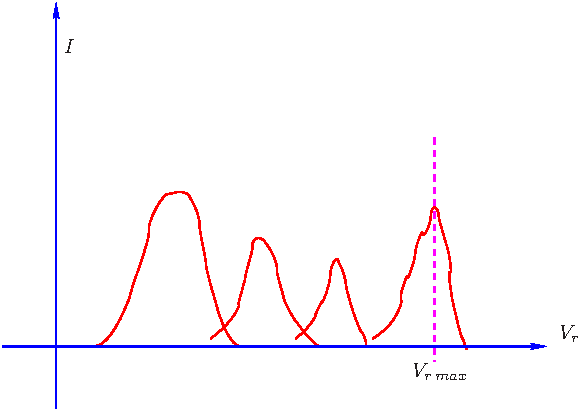
\includegraphics[width=10cm]{../figures/vmax.pdf}
\end{center}
\caption{There can be multiple velocity components in the observed spectrum, each peak corresponds
to a cloud with some relative velocity.}
\label{fig:vmax}
\end{figure}
We now assume that clouds at larger distances from the center move with equal
or lower speed than clouds closer to the center, as expected from standard
Keplarian motion (see Appendix. \ref{sect:kepler}).  In this case, the {\bf
largest velocity component}, $V_{\rm r,max}$, comes from the cloud {\bf at the
tangential point} ({\bf T}), since the maximum possible projected velocity
happens when the projection angle is 0.  For a cloud at the tangent point we
see from Fig. \ref{fig:galgeom} that the cloud location is given by 
\begin{equation}
	R = R_0 \sin l.
	\label{eqn:rotR}
\end{equation}

This simplifies equation \ref{eqn:vrel2} so that, at the tangential point, we
have: 
\begin{equation}
V = V_{r,max} + V_0 \sin l .
\label{eqn:rotV}
\end{equation}

We may now use SALSA to measure $V_{\rm r,max}$ at different $l$ in the first
quadrant.  Using equations \ref{eqn:rotR} and \ref{eqn:rotV} we may then
calculate the rotation curve $V(R)$. We note that even though we only measure
in the first quadrant, we can measure velocities of clouds both closer to, and
further away from, the glactic center than the Sun.  It is therefore reasonable
to assume the measured rotation curve to be valid also in the other three
quadrants.

\subsection{Measure the rotation curve with SALSA}
\label{sect:SALSArot}
After reading the previous section you should have an idea about how to measure
the rotation curve of the Milky Way using SALSA. Instructions for how to
operate the telescope are given in another document called the \emph{SALSA
users manual}, available at the SALSA website.
Once you have obtained spectra
at a few selected longitudes, extract the maximum velocity of each spectrum and
plot the rotation curve.   
The simplest way is to use the cursor to inspect the spectrum directly in the
control program, but you can also use more advanced tools such as
Matlab.Instructions for how to extract velocity information from the spectra
can also be found in the \emph{SALSA users manual}.
To make the final plot of the rotation curve you may use your favourite
plotting program.  A simple free solution is to use the \emph{Excel-like}
program \emph{LibreOffice Calc}, where you can put your calculated
values of V and R in a spreadsheet and then use the {\tt xy-chart} 
to plot the data. Your final plot should look similar to Fig. \ref{fig:rotfinal}.
Note that the rotation curve is almost flat! This is an indirect evidence
for dark matter in our galaxy. You may also want to compare with the results in 
Appendix \ref{app:rotcurves}.

\begin{figure}[t]
\begin{center}
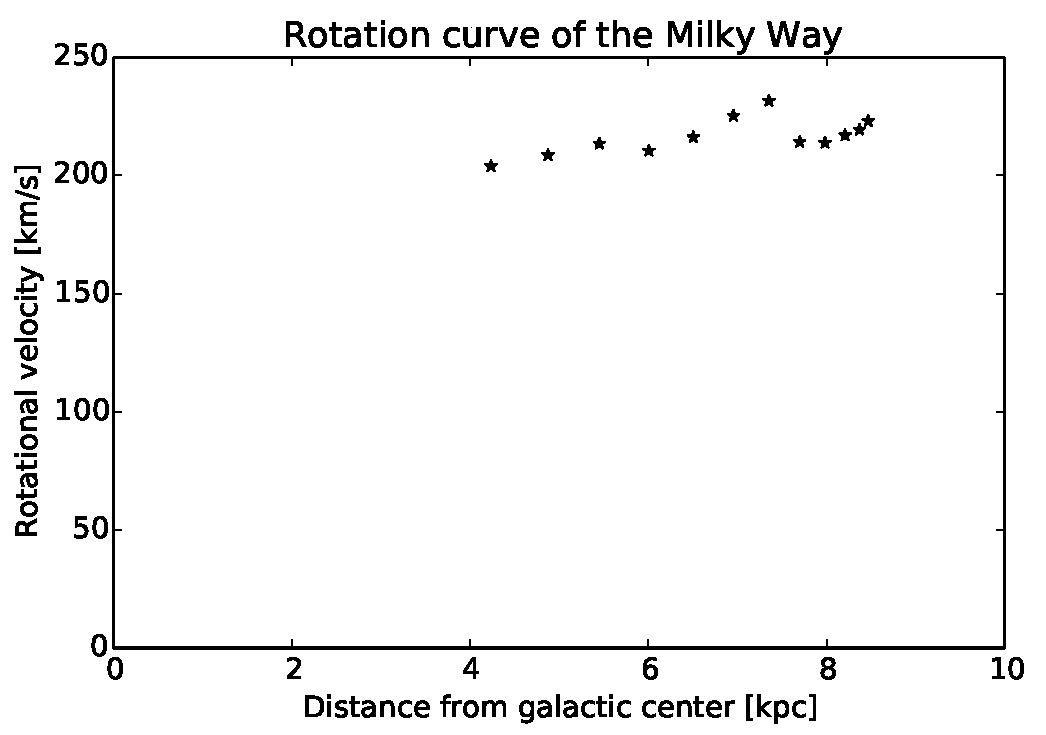
\includegraphics[width=0.7\textwidth]{../figures/SALSA_rotcurve.pdf}
\caption{Example of a rotation curve measured with SALSA.}
\label{fig:rotfinal}
\end{center}
\end{figure}

\section{Mapping the Milky Way}
\label{sect:map}
Now we would like to find out {\em where} is the HI gas that we have detected.
Let us therefore return to eqn. \ref{eqn:vrel2}.  When finding the rotation
curve, we used only the maximum velocity component in the spectrum, and assumed
that it came from gas at the tangential point.  This assumption made it
possible to solve eqn. \ref{eqn:vrel2} in the first quadrant.  Now, we shall
use  {\em all the velocity components} that we see in our spectra, and we want
to be able to map in all observable directions, not only in the first quadrant. 
We can now use our knowledge about the rotation curve obtained in the Sect. \ref{sect:SALSArot}.
Motivated by the shape our measured rotation curve we now assume that the gas in our Milky Way 
obeys {\em differential rotation}, i.e. the rotational speed is
constant with radius and is the same as the rotational speed of the Sun, i.e.
\begin{equation}
	V(R) = {\rm constant} = V_0.
\end{equation}
With this assumption, eqn. \ref{eqn:vrel2} simplifies to 
\begin{equation}
V_r = V_0\sin l \left( \frac{R_0}{R} -1 \right).
\end{equation}
This equation can be re-written as an expression for the cloud distance $R$ as
a function of known (or observable in the case of $V_r$) quantities as
\begin{equation}
\boxed{
R = \frac{R_0 V_0 \sin l}{V_0 \sin l + V_r}.
}
\label{eqn:Rmap}
\end{equation}

Now we would like to make a map of the Milky Way and place the
position of the cloud that we have detected.  From our measurement of
the radial velocity $V_r$ we have just calculated the distance of the
cloud to the Galactic center, $R$, and we know in which direction we
have observed (the Galactic longitude $l$). 

Please note that if you observe in Quadrants II or III, then the position of
the emitting gas clouds can be determined uniquely. But, if observing in
Quadrants I or IV, there may be {\em two possible locations} corresponding to
given values of $l$ and $R$: closer to us than the tangential point $T$ (the
actual point {\bf M} on the figure), or farther away, at the intersection of
the {\bf ST} line and the inner circle (see Fig. \ref{fig:galgeom}).
{\bf You may want to make a drawing to convince yourself that
this is true.}

This distance ambiguity can also be shown mathematically. Let $r$ denote the
distance from the Sun to the cloud, i.e. the distance between the points {\bf
S} and {\bf M} in  Fig.  \ref{fig:galgeom}. Using the law of cosines on the triangle
{\bf CSM} we obtain the following relation:
\begin{equation}
R^2 = R_0^2 + r^2 - 2 R_0 r \cos l.
\end{equation}
This is a second-order equation in $r$, which has two possible solutions. If we
denote these solutions $r=r_{+}$ and $r=r_{-}$, we can write the solutions as
\begin{equation}
\boxed{
r_\pm = \pm \sqrt{R^2 - R_0^2 \sin^2 l} + R_0\cos l .
}
\label{eqn:rpm}
\end{equation}

In Quadrants II or III, $R$ is always larger than $R_0$ and $\cos l <0$,
meaning there is one and only one positive solution, $r_+$. The negative
solution is not meaningful (we are not looking through the Earth) and should be
discarded. In Quadrants I or IV, there may be two positive, and therefore
possible, solutions. In cases with two possible solutions it is not possible to
determine which one is the correct one without additional observations.  To
resolve this ambiguity, one can observe again towards the same galactic
longitude but towards a small (a few degrees) non-zero galactic latitude.  If
the ambigous cloud is far away, it should no longer be seen. If the cloud is
close, it should still appear even if observing slightly out of the plane. 
Some experimenting may be necessary here to find out the appropriate
galactic latitude.

\subsection{Converting from $r$ and $l$ to Carteesian coordinates} 
For plotting it may be inconvenient to use the coordinates $r$ (distance to
cloud from the Sun) and $l$ (galactic longitude) to describe the cloud
positions. Instead it is usually more convenient to transform to a Carteesian
system of perpendicular coordinates $x$ and $y$.  To convert to $x-y$
coordinates we need to relate them to $r$ and $l$.  

You are probably familiar with \emph{polar coordinates}, usually defined as
\begin{equation}
\left\{ 
\begin{array}{l}
x=r \cos \theta \\
y=r \sin \theta \\
\end{array}
\right.
\label{eqn:polar}
\end{equation} 
where $r$ is the distance from the origin and $\theta$ is the rotation angle, and 
$x$ and $y$ are Carteesian coordinates. 

It is clear that polar coordinates are very similar to our $r$, $l$-system,
as is also evident when plotting both together in Fig. \ref{fig:polar}.
\begin{figure}[ht]
\begin{center}
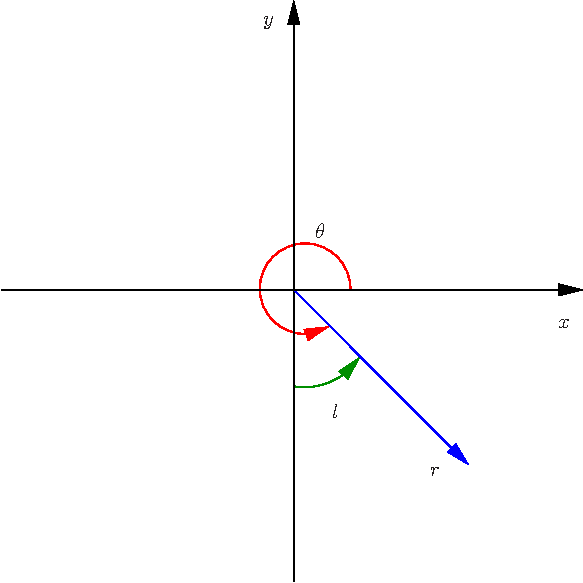
\includegraphics[width=0.5\textwidth]{../figures/coordinate.pdf}
\caption{Illustration of polar ($r$,$\theta$) versus Galactic
  ($r$,$l$) coordinates.}
\label{fig:polar}
\end{center}
\end{figure}
We find that $\theta=270^\circ +l$, or $\theta=l-90^\circ$. This means that we can convert our positions given as $r$,
$l$ to Carteesian $x-y$ coordinates by:
\begin{equation}
	\boxed{
\left\{ 
\begin{array}{l}
	x=r \cos (l-90^\circ) \\
	y=r \sin (l-90^\circ) \\
\end{array}
\right.}
\label{eqn:rpmtocart}
\end{equation} 
This format is usually the most convenient to plot the positions. 

\subsection{Make a map with SALSA}
\label{sect:SALSAmap}
After reading the previous section you should have an idea about how to
construct a map from measured velocities. The measurements are done in the same
way as you did in Sect. \ref{sect:SALSArot}, but now you do not have to measure
in the first quadrant. Also, you should extract all velocity components in your
spectra, not only the maximum one.  Again, instructions for how to operate the
telescope are given in another document called the \emph{SALSA users manual},
available at the SALSA website.  The simplest way to obtain velocities from a
spectrum is to use the cursor to inspect the spectrum directly in the control
program, but you can also use more advanced tools such as Matlab. Instructions
for how to extract velocity information from the spectra can also be found in
the \emph{SALSA users manual}.

Once you have a list of measured velocities for multiple longitides you
can use eqn. \ref{eqn:rpm} to find the position of the clouds. Note that
observations in Quadrants I or IV may need additional observations
to resolve possible distance ambiguities, as discussed in the previous section.

To make the final map you may use your favourite plotting program.  Again, a
simple free solution is to use the \emph{Excel-like} program \emph{LibreOffice
Calc}, where you can put your calculated positions (x,y) in a spreadsheet and
then use the {\tt xy-chart} to plot the data.  Your final map may look similar
to Fig. \ref{fig:rotfinal}, although it will depend on in which directions you
have been observing.  You may also want to compare with the map on the cover
page of this document.

\begin{figure}[t]
\begin{center}
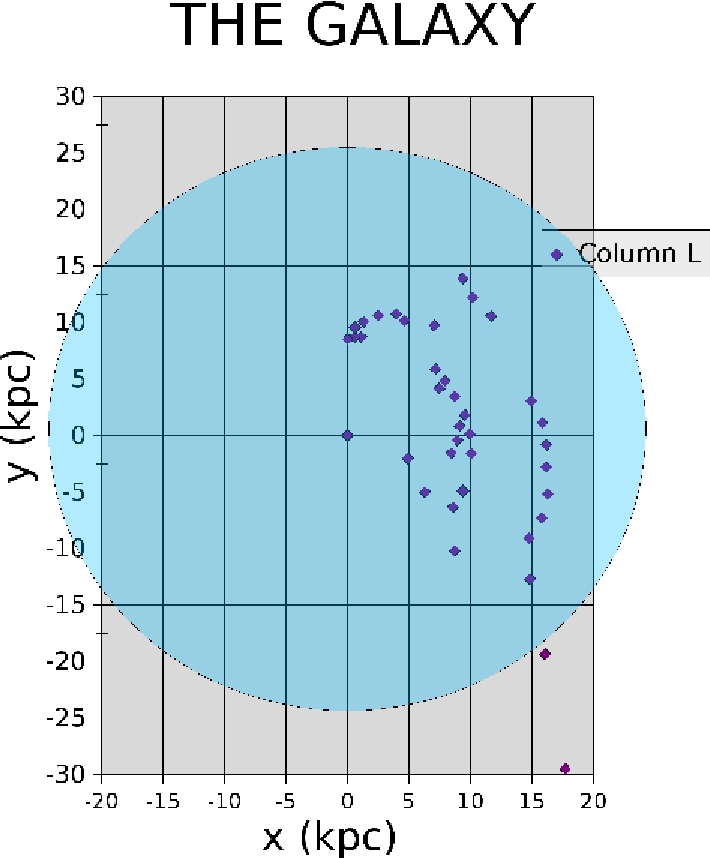
\includegraphics[width=0.6\textwidth]{../figures/galaxopenoffice1.pdf}
\caption{Snapshot of the $xy$-chart in OpenOffice.  You can clearly
  see the spiral arms in the Galaxy.  The blue circle represents the
  area of the Galaxy, which has diameter of 50~kpc.}
\label{fig:mapfinal}
\end{center}
\end{figure}
